\documentclass[aspectratio=169]{beamer}


\usepackage[utf8]{inputenc}
\usepackage{amsmath}
\usepackage{amsfonts}
\usepackage{amssymb}
\usepackage{graphicx}
\usepackage{ragged2e}  % `\justifying` text
\usepackage{booktabs}  % Tables
\usepackage{tabularx}
\usepackage{tikz}      % Diagrams
\usetikzlibrary{calc, shapes, backgrounds}
\usepackage{amsmath}
\usepackage{amssymb}
\usepackage{dsfont}
\usepackage{url}       % `\url
\usepackage{listings}  % Code listings
\usepackage[T1]{fontenc}


\usepackage{theme/beamerthemehbrs}

\author[Veeramacheneni]{Lokesh Veeramacheneni}
\title{Out-of-Distribution Detection in 3D Semantic Segmentation}
\subtitle{Master Thesis}
\institute[HBRS]{Hochschule Bonn-Rhein-Sieg}
\date{September 02, 2022}
\subject{Test beamer}

% leave the value of this argument empty if the advisors
% should not be included on the title slide
\def\advisors{Prof. Dr. Paul G Pl\"{o}ger, Prof. Dr. Matias Valdenegro Toro, Prof. Dr. Sebastian Houben}

\thirdpartylogo{images/DFKI.png}


\begin{document}
{
\begin{frame}
\titlepage
\end{frame}
}

\section{Introduction}
% 1. Discuss about what is OOD
% and need for OOD along with some real life examples
% 2. Explain about 3D Semantic segmentation task
\begin{frame}{Out-of-Distribution detection}
 \begin{columns}
    \begin{column}{0.5\textwidth}
     
    \end{column}
    \begin{column}{0.5\textwidth}
     \begin{figure}
         \centering
         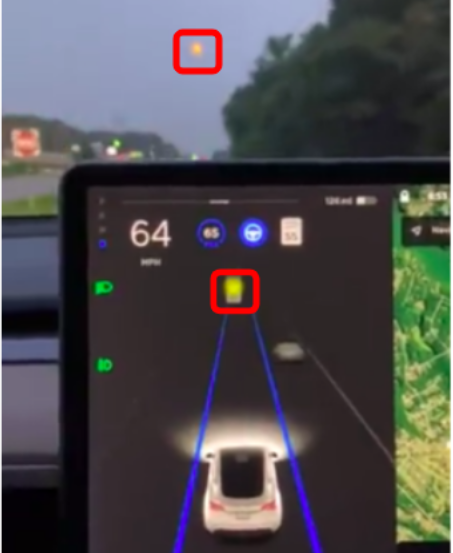
\includegraphics[scale=0.25]{images/Tesla_ex_moon.png}
         \caption{Caption}
         \label{fig:my_label}
     \end{figure}
    \end{column}
 \end{columns}
\end{frame}
\section{Methodology}
% Explain about what are the requirements for setup one by one such as
% Datasets & benchmarking, OOD method, 3D Model, Uncertainty methods, Evaluation metrics
\section{Experiments \& Results}
% Arrange the experiments and explain the results here
\section{Conclusion}
\begin{frame}{Lessons Learned}
    Learning's during the duration of the thesis are
    \begin{enumerate}
        \item Training and evaluation of 3D DNNs are time consuming and resource intensive.
        \item Finding the proper prior for Flipout layers is hard and currently we use brute force to find the best fitting prior.
        \item OOD benchmarking require in depth analysis of datasets like studying the structural similarties in the datasets and also color spectrum.
        \item LiDAR datasets have large memory requirements especially for the preprocessing and metric computation.
        \item Getting 100\% OOD detection performance is not possible with the post-hoc methods used as some points in the ID dataset also have low probability scores.
    \end{enumerate}
\end{frame}
\begin{frame}{Conclusion}
    
\end{frame}
\begin{frame}{Future Work}
    This thesis can be extended in the following ways.
    \begin{enumerate}
        \item This thesis is limited to only point based models, this can be extended to graph and projection based models.
        \item The datasets involved are only static datasets and this thesis study can be further extended to other type of datasets such as synthetic and sequential datasets.
        \item Since this thesis utilzes post-hoc threshold methods for OOD detection. Other methods such as Mahalanobis distance based OOD detection \cite{lee2018simple_mahalanobis} or MetaSeg \cite{MetaSeg} can be added as an extension to this thesis.
    \end{enumerate}
\end{frame}
\begin{frame}{References}
    \bibliographystyle{plain}
    \bibliography{bibliography.bib}

\end{frame}

%\section{First section}
%\subsection{A subsection}

%\begin{frame}{Jabberwocky}
%      \framesubtitle{Lewis Carroll}%
%      \begin{tikzpicture}[overlay,remember picture]
%        \node[anchor=south east,xshift=-30pt,yshift=35pt]
%          at (current page.south east) {
%            %\includegraphics[width=35mm]{resources/jabberwocky-light}
%          };
%      \end{tikzpicture}%
%      'Twas brillig, and the slithy toves\\
%      Did gyre and gimble in the wabe;\\
%      All mimsy were the borogoves,\\
%      And the mome raths outgrabe.\\\bigskip

%      “Beware the Jabberwock, my son!\\
%      The jaws that bite, the claws that catch!\\
%      Beware the Jubjub bird, and shun\\
%      The frumious Bandersnatch!”\\
%\end{frame}

%--- Next Frame ---%
\begin{frame}{What is OOD Detection?}
    \begin{figure}
        \centering
        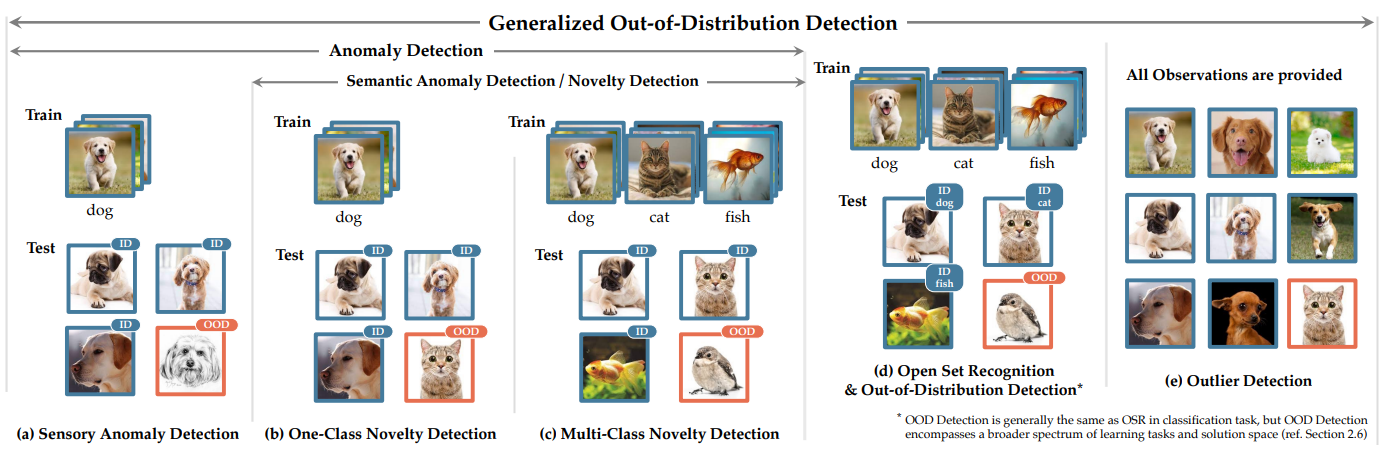
\includegraphics[scale=0.3]{images/OOD_ex_new.png}
        \caption{Generalized Out-of-Distribution Detection: A Survey}
        \label{fig:my_label}
    \end{figure}
\end{frame}


\end{document}
